\chapter{Lösungsidee}

\section{Das Spieldesign}

Das \textit{CZGame} ist ein Point-and-Click Computerspiel, welches im Carl-Zeiss-Gymnasium
Jena spielt. Das Gameplay besteht Hauptsächlich aus dem Spielen von Minigames, also kleinen
spielerischen Aktivitäten innerhalb des Spiels, und aus \glqq{}mündlichen Prüfungen\grqq{}. Bei letzteren handelt es sich um Duelle mit den Lehrkräften der verschiedenen Fachschaften der
 Schule. Diese müssen gewonnen werden mithilfe verschiedener Gegenstände, die durch das Gewinnen der Minigames erhalten werden.

Die Minigames und Duelle sind an verschiedenen Orten innerhalb der Spielwelt platziert,
welche dem Schulgebäude nachempfunden ist: Sowohl eine vereinfachte Version der Gänge
als auch einige begehbare Räume wurden im Spiel umgesetzt und gestaltet.

\begin{figure}[ht]
	\centering
	\begin{minipage}[b]{0.45\textwidth}
		
\includegraphics[scale=0.41]{bilder/Foyer.png}
		\caption{Das Foyer bildet den Ausgangsort des CZGame}
		\label{abb:foyer}
	\end{minipage}
	\hfill
	\begin{minipage}[b]{0.45\textwidth}
		\includegraphics[scale=0.41]{bilder/Hausmeisteraum.png}
		\caption{Im Raum des Hausmeisters ist ein Modell der Schule zusehen}
		\label{abb:hausmeister}
	\end{minipage}
\end{figure}

Da das Spiel im Pixelartdesign entstehen sollte, musste ein geeignetes Programm genutzt werden um das Format der Graphik digital und in Pixeln zu implementieren. Das herkömmliche Format eines Computerbildschirms beträgt standardmäßig 16 zu 9. Da das CZGame als PC-Spiel entworfen werden sollte wurde ein rechteckiges Format der Größe 240 zu 135 Pixeln gewählt, das diesem Verhältnis entspricht.


Als Programm wurde das kostenlose und qualitativ hochwertige Onlinetool \emph{Pixelart} verwendet.  
Innerhalb der Gruppe \emph{Graphikdesign} wurde die Arbeit zum erstellen der Hintergrundgraphiken aufgeteilt. Durch die kollektive Zusammenarbeit beim erstellen der Bilder, kommt es im Endergebnis zu einer großen Vielfalt an Farben und Formen, die die Freude am Spiel fördern sollen. Da jeder die Möglichkeit hatte selbst schulspezifische Mottos in die Hintergründe einzubringen, sorgt jeder Raum ganz individuell für eine Überraschung.

Die Gruppe \emph{Graphikdesign} stand während den Arbeiten an den Bilddateien in starkem Austausch mit der Gruppe \emph{Item- \& Charakterdesign} so wie mit den Verantwortlichen für das Erstellen von Minigames. Unter anderem musste das Größenverhältnis der Charaktere und Spielerfiguren auf die Größe der Räume angepasst werden. 

Für das Design der einzelnen Spielerfiguren und der Figuren des Lehrkörpers wurde aufgrund der guten Kompatibilität einzelner Bilddateien untereinander ebenfalls \emph{Pixelart} verwendet. So konnte später in der Java-Implementierung ermöglicht werden, das zu Beginn des Spiels jeder Spieler seine individuelle Spielerfigur erstellen kann, dies erhöht das eigene Spielvergnügen und gibt dem Spiel eine persönliche Note.





\section{Der Spielaufbau}

Das CZGame sollte grundsätzlich die Form eines Point-and-Click-Spiels erhalten. Während der Spieler sich über dafür vorgesehene Pfeile durch das Schulgebäude bewegt, sollte die Möglichkeit eines sogenannten Minigames oder einer Challenge, ähnlich einer mündlichen Prüfung mit einem Mitglied des Lehrkörpers, bestehen. Das Wechseln der Räume erfolgt über Standbilder, in denen die Figur durch 

Die Minigames wurden von einem eigens dafür bestimmten Team entworfen und in Java implementiert. 
Dabei sollte in jedem der folgenden Fächer die Möglichkeit eines Minigames und einer mündlichen Prüfung bestehen:
\begin{itemize}
    \item Fachschaft Biologie
        \begin{itemize}
        \item Das Minigame der Fachschaft Biologie ähnelt in seine Grundzügen dem Pflanzentestat am Carl-Zeiss-Gymansium Jena. Um eine möglichste Originaltreue der zuerkennenden Pflanzen zu schaffen wurden über 30 Pflanzen als erkennbare Graphik gepixelt und in Java implementiert.
        \end{itemize}
    \item Fachschaft Chemie
        \begin{itemize}
        \item Das Chemie Minigame entspricht der bekannten Form eines Water-Sort-Puzzles.
        \end{itemize}
    \item Fachschaft Informatik
        \begin{itemize}
        \item In der Fachschaft Informatik wird zum Lösen des Minigames Kenntnis von Grundlegenden informatischen Schaltarten vorausgesetzt. Da hier auf der Basis von Schaltungen auf das entsprechende Schaltzeichen zurück geschlossen werden muss.
        \end{itemize}
    \item Fachschaft Mathematik
        \begin{itemize}
        \item Das Lösen von Tangramfiguren der Hauptteil der Mathematikminigames.
        \end{itemize}
    \item Fachschaft Physik
        \begin{itemize}
        \item Um einen Ball auf eine vorgegebene Stelle zu positionieren muss im Minigame der Fachschaft Physik der Zusammenhang von Kräften und deren Vektoren erkannt und angewendet werden. 
        \end{itemize}
\end{itemize}

Jedes Minigame sollte zudem aus drei unterschiedlichen Leveln bestehen, mit einem aufsteigenden Schwierigkeitsgrad von Eins bis Drei. Beim erfolgreichen Lösen eines solchen Levels, gewinnt der Spieler Items, die sich als Symbole für die zuvor genannten Fachschaften herausstellen.

Alle Items sind gleichwertig und können als unterstützendes Mittel während einer mündlichen Prüfung in jedem Fach eingesetzt werden. Das Sammeln der Items sowie der Einsatz erfolgt automatisch oder über dafür vorgesehene Buttons.


In der gesamten Arbeit soll auf Abbildungen verwiesen werden (siehe Abbildung \ref{abb:beispiel}) und gegebenenfalls hilfreiche Zitate eingefügt werden.\newline
Wörtliche Rede wird in Latex zwischen \verb|"`| und \verb|"'| gesetzt. 

\begin{quote}
 "`\blindtext"'\footnote{Heinemann, 1998, S.\,280}
\end{quote}

\section{Die Spiel-Engine}
Um die Komponenten des Spiels sinnvoll und geordnet umsetzen zu
können, wird eine \textit{Spiel-Engine} benötigt, also ein
Grundgerüst aus Code, welches das Einbinden von Grafik, Audio sowie
das implementieren der Spiel-Logik vereinfacht sowie vereinheitlicht.

Die Engine des CZGame sollte folgende Funktionen
beinhalten:

\begin{itemize}
	\item Das Erstellen von \textit{Spiel-Objekten}, also
	frei über den Bildschirm bewegliche Bilder oder Figuren,
	welche optional noch beliebigen Code ausführen können.
	\item Das Zusammenfassen von Spiel-Objekten in \textit{Szenen},
	sodass die Objekte einfach gemeinsam verwaltet werden können.
	\item Das Anzeigen mehrere Szenen übereinander, sodass z.B.
	eine Szene, welche eine Textbox enthält über der Szene mit
	der Spielfigur und dem Hintergrund eingeblendet werden kann.
	\item Das eigentliche \glqq{}Zeichnen\grqq{} oder \textit{Rendern} der Spielgrafiken
	sowie das geordnete Ausführen von Szenen- und Spiel-Objekt-spezifischem
	Code in einem Festen Intervall von 60Hz.
	\item Das Abspielen beliebiger Audio-Dateien (\textit{Sounds})
	sowie die Steuerung von deren Wiedergabe.
	\item Das Zusammenfassen verschiedener Sounds zu \textit{Sound-Gruppen},
	um mehrere Sounds gemeinsam pausieren, starten oder stoppen zu können.
	So beinhaltet jede Szene eine eigene Sound-Gruppe, sodass die in ihr
	abgespielten Sounds beim Ausblenden bzw. Entfernen der Szene einfach
	und einheitlich gestoppt werden können.
\end{itemize}


\subsection{Hauptschleife} \label{idee:engine:hauptschleife}

Um die Grafik und Logik des Spiels mit einer Frequenz von 60Hz
auszuführen, wird eine in der Spieleprogrammierung häufig
genutzte Methode angewendet. Die Grundidee ist es, in einer
Endlosschleife einen Zähler jeweils um die seit dem letzten
Durchlauf der Schleife vergangene Zeit zu erhöhen. Erreicht der
Zähler die Zeitmenge, nach welcher ein Durchlauf der Spiellogik
ablaufen sollte, in diesem Fall also $\frac{1}{60}s$, wird dies
getan und der der Zähler wieder um ebendiese Zeiteinheit verringert.

Ein solcher Durchlauf der Spiellogik sowie das Rendern der Grafik
wird als \textit{Frame} bezeichnet.


\subsection{Klassen}

Grundsätzlich sollte es für Spiel-Objekte und Szenen jeweils eine
Basis-Klasse geben, die beim Umsetzen von Spielkomponenten von einer
neuen Unterklasse erweitert wird, welche dann mindestens einen eigenen
Konstruktur bereitstellt sowie optional Methoden der Elternklasse
überschreibt, um eigene Logik zu implementieren.


\subsection{Grafik und Eingabe} \label{idee:engine:grafik-eingabe}

\begin{sloppypar}

Zum Laden und Speichern von Bildern bietet Java die Methoden
und Klassen \texttt{javax.imageio.ImageIO.read} sowie
\texttt{java.awt.Image} bzw. \texttt{java.awt.image.BufferedImage}.

Um Tastatur- und Mauseingaben zu verarbeiten sowie Grafik
anzuzeigen, wird das \texttt{Java Swing Framework} verwendet.

Mit der Klasse \texttt{javax.swing.JFrame} wird das Fenster
erstellt in welchem das Spiel läuft. \texttt{Swing} bietet eine große
Bandbreite an Komponenten für grafische Oberflächen, von denen
jedoch hauptsächlich \texttt{javax.swing.JPanel} verwendet wird,
ein generischer Behälter für andere Komponenten. Eine Instanz von
diesem wird zum Fenster hinzugefügt. Durch das Überschreiben der
\texttt{paintComponent}-Methode von \texttt{JPanel} kann eigener
Rendering-Code hinzugefügt werden, im Fall des CZGame also
das Zeichnen der Szenen und ihrer Objekte. Dieses kann durch
Aufrufen der \texttt{repaint}-Methode dann manuell ausgelöst werden,
um die Grafik eben mit einer Frequenz von 60Hz zu aktualisieren.

Um Eingaben zu erhalten, werden die Interfaces \texttt{java.awt.event.KeyListener}
sowie \texttt{java.awt.event.MouseListener} implementiert und mit
der Methode \texttt{addKeyListener} bzw. \texttt{addMouseListener}
beim Spielfenster registriert. Tastatur- und Mauseingaben werden
so über Methoden wie \texttt{keyPressed} oder \texttt{mousePressed}
der Interfaces mitgeteilt. Da die Aufrufe dieser Methoden selbstständig
durch \texttt{Swing} erfolgen und somit nicht synchron mit dem
Rest der Spiellogik laufen, werden diese Interfaces von einer einzelnen
Klasse implementiert, welche dann die Zustände der Tasten mithilfe der
auf parallelen Zugriff spezialisierten Datenstruktur
\texttt{java.util.concurrent.ConcurrentHashMap} speichert sowie
Zugriff darauf gewährt.
\end{sloppypar}


\subsection{Sound}

\begin{sloppypar}
Java bietet über die \texttt{Java Sound API} eine vorgefertigte Schnittstelle zum Laden und Abspielen von Audiodateien.
\par Die am einfachsten zu verwendende Klasse dieser Schnittstelle ist
\texttt{javax.sound.sampled.Clip}. Diese bietet Methoden wie \texttt{setMicrosecondPosition}, \texttt{start} und \texttt{stop}, mit
welchen die Wiedergabe einfach gesteuert werden kann. Der entscheidende
Nachteil der \texttt{Clip}-Klasse ist jedoch, dass sie die gesamten Audiodaten auf einmal in den Speicher lädt. Das ist bei kleinen, wenige Sekunden langen Audiodateien kein Problem, jedoch für Musikstücke, welche mehrere Minuten dauern, ungeeignet. 
\par Um dieses Speicherproblem zu lösen, müssen die Audiodaten \textit{gestreamt},
also in kleinen Stücken in den Speicher geladen, abgespielt und wieder
verworfen werden. Es befindet sich also immer nur eine kleine Teilmenge der Gesamtaudiodaten im Speicher.
\par Zur Umsetzung des Streamens stellt die Java-Standardbibliothek die Klassen \texttt{AudioInputStream} und \texttt{SourceDataLine} bereit. Erstere ermöglicht es, eine Audiodatei zu öffnen und zu
dekodieren, also die enthaltenen Audiodaten zu lesen. Im zweiten
Schritt müssen die gelesenen Daten an eine Instanz von \texttt{SourceDataLine} übergeben werden, welche diese dann abspielt. Dazu wird deren \textit{write}-Methode verwendet.
\end{sloppypar}


\section{Grafikdesign}
\input{texte/03_loesungsidee-Grafikdesign.tex}

\section{Kampfkonzept}
Im Kampf geht es darum, dass der Schüler sich gegen den Lehrer beweisen muss. Dafür werden Items unterschiedlicher Level benutzt, die dann gegenseitig eingesetzt werden, um sich Lebenspunkte abziehen zu können.\\
Dafür ist erst der Schüler und dann der Lehrer am Zug. Das Ganze wechselt sich ab, bis entweder der Schüler aufgibt oder einer der beiden keine Lebenspunkte mehr hat.\\
Wenn der Schüler am Zug ist, kann er sich eins seiner Items aus seinem Inventar aussuchen, die er im Vorfeld durch die Minigames gesammelt hat. Der Lehrer kann dann mit einem seiner Items darauf reagieren oder nichts tun.\\
Danach ist der Lehrer am Zug. Er wählt sich auch eins seiner Items aus, auf das der Schüler dann wiederum reagieren kann oder aufgibt.\\
Der Schaden wird folgendermaßen berechnet: Die Items haben Level zwischen 0 und 2. Der Schaden, der durch ein Item erzielt wird, ist das Level + 1.\\
Die erste Partei wählt dann eins ihrer Items aus, welches das Level $l_1$ hat. Die zweite Partei kann sich dann ein Item mit dem Level $l_2$ aussuchen. Die Schadenswerte sind $s_1 = l_1 + 1$ bzw. $s_2 = l_2 + 1$.\\
Es wird die Differenz der beiden Schadenswerte betrachtet: $d = s_1 - s_2$.\\
Falls diese größer als null ist, erhält die zweite Partei Schaden in Höhe der Differenz, weil sie mit einem Item reagiert, welches ein kleineres Level als das erste hatte, also schlechter ist.\\
Wenn die $d\leq 0$ ist, erhält die zweite Partei keinen Schaden, weil sie mit einem Item reagiert hat, welches gleich gut oder besser ist.\\
Der Schaden wird dann von den Lebenspunkten abgezogen.\\
Wenn dann eine der beiden Parteien 0 Lebenspunkte (oder weniger) hat, ist der Kampf vorbei.\\
Sollte der Schüler gewonnen haben, ist der Lehrer besiegt und, wenn alle Lehrer besiegt sind, ist das Spiel gewonnen.\\


\section{Minigames}
Jedes Minispiel ist aus drei Leveln aufgebaut, welche progressiv schwerer werden.
So dient das erste Level als Einführung in die Mechaniken des jeweiligen Minispiels.
Das zweite Level kann als \glqq standard\grqq{}-Schwierigkeitsgrad verstanden werden und im Dritten können die Spielenden dann ihre erlernten Fähigkeiten in schwierigen Herausforderungen unter Beweis stellen.
Nach dem erfolgreichen Beenden eines Levels erhält die Spielfigur ein Item, welches dann im Kampf verwendet werden kann.
Diese Items hängen von der Fachschaft und dem Schwierigkeitsgrad ab.
Die Stärke der Items skaliert also mit der Schwierigkeit des beendeten Levels. 
Da das Bearbeiten schwererer Level länger dauert, wird dies dementsprechend belohnt.\\
Im Allgemeinen soll jedes Minispiel mit einer Auswahl des Schwierigkeitsgrades beginnen, welche auch wieder verlassen werden kann, wenn sich doch gegen das Spielen entschieden wird.
Jedes Level bietet zusätzlich noch die Möglichkeit, zur Auswahl zurückzukehren.
Nach dem Abschließen des selbigen ist es ebenfalls möglich, das Level neu zu starten.


\subsection{Informatik}

Grundlegende Idee dieses Minispiels ist das \glqq Bauen\grqq{} eines Schaltkreises aus vorgegeben Logikgattern, der vorgegebene Bedingungen erfüllen soll.
Die Spielenden haben gewonnen, wenn das richtige beziehungsweise die richtigen Gatter ausgewählt wurden.
Es kann nur das erste Level verloren werden, worauf später noch eingegangen wird.\\
Die Level der Fachschaft Informatik bestehen jeweils aus zwei wesentlichen Komponenten:
Zunächst gibt es einen Schaltkreis, welcher aus Tastern, mit \glqq{}?\grqq{} verdeckten Logikgattern sowie Lämpchen aufgebaut ist.
Die zweite Komponente bilden verschiedene Logikgatter, aus welchen das im Schaltkreis verdeckte bzw. die im Schaltkreis verdeckten ausgewählt werden müssen.

\begin{figure}[H]
	\centering
	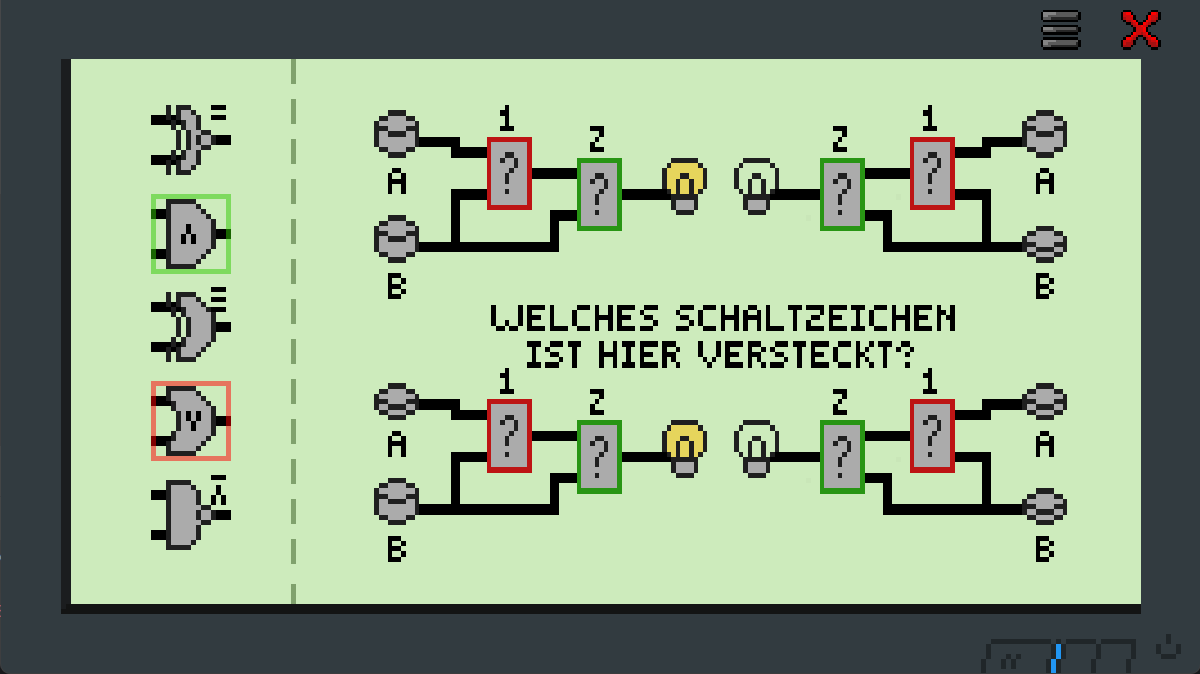
\includegraphics[width=.7\textwidth]{bilder/MinispielInformatik.png}
	\caption{Level 2 des Minispiels der Fachschaft Informatik}
	\label{fig:mginf}
\end{figure}

Verschiedene Schwierigkeiten werden auf zwei Weisen ermöglicht:

\begin{itemize}
    \item Die Anzahl an Logikgattern, aus denen ausgewählt werden kann, erhöht sich mit jedem Schwierigkeitsgrad.
            So sind es im ersten Level 4, im zweiten Level 5 und im dritten Level 6 Logikgatter, welche zur Auswahl stehen.
    \item Die Komplexität des Schaltkreises sowie die Anzahl an verdeckten Gattern ändern sich dem Schwierigkeitsgrad entsprechend.
\end{itemize}

Jedes Level verwendet außerdem, im Sinne der Variabilität, drei verschiedene Schaltkreise, aus denen bei jedem Minispiel-Start einer zufällig gewählt wird.

\subsubsection{Level 1}

Bei den Schaltkreisen des ersten Levels fehlt jeweils nur ein Logikgatter, das zwei Eingänge mit einem Ausgang verbindet.
Gesucht wird also das Logikgatter $G \in \{\land , \lor , \overline{\land}, \overline{\lor}, \veebar, \overline{\veebar}\}$\footnote{$\land = AND,\ \lor = OR,\ \overline{\land} = NAND,\ \overline{\lor} = NOR,\ \veebar = XOR,\ \overline{\veebar} = XNOR$}, welches folgende Bedingungen erfüllt:

\begin{align*}
    x_1 G x_2 = y
\end{align*}

Dadurch, dass jeder Schaltkreis zwei Eingänge und einen Ausgang besitzt, ergeben sich vier mögliche Zustände, die in Form einer Wahrheitswerttabelle dargestellt werden können.
Für die Rätsel des ersten Levels wurden folgende Tabellen festgelegt:

\begin{table}[H]
    \centering
    \begin{minipage}{.33\textwidth}
        $G = \land$\\
        \vfill
        \begin{tabular}{|c|c|c|} 
            \hline
            $x_1$ & $x_2$ & $y$ \\
            \hline\hline
            $0$ & $0$ & $0$ \\
            $0$ & $1$ & $0$ \\
            $1$ & $0$ & $0$ \\
            $1$ & $1$ & $1$ \\
            \hline
        \end{tabular}
    \end{minipage}
    \hfill
    \begin{minipage}{.32\textwidth}
        $G = \lor$\\
        \vfill
        \begin{tabular}{|c|c|c|} 
            \hline
            $x_1$ & $x_2$ & $y$ \\
            \hline\hline
            $0$ & $0$ & $0$ \\
            $0$ & $1$ & $1$ \\
            $1$ & $0$ & $1$ \\
            $1$ & $1$ & $1$ \\
            \hline
        \end{tabular}
    \end{minipage}
    \hfill
    \begin{minipage}{.33\textwidth}
        $G = \overline{\land}$\\
        \vfill
        \begin{tabular}{|c|c|c|} 
            \hline
            $x_1$ & $x_2$ & $y$ \\
            \hline\hline
            $0$ & $0$ & $1$ \\
            $0$ & $1$ & $1$ \\
            $1$ & $0$ & $1$ \\
            $1$ & $1$ & $0$ \\
            \hline
        \end{tabular}
    \end{minipage}
    \caption{Wahrheitswerttabellen für Level 1 des Informatik-Minispiels}
    \label{tab:wwt01}
\end{table}

Diese Tabellen werden den Spielenden, aufgrund der ansprechenderen Gestaltung, in Form einer Abbildung präsentiert, welche die vier Zustände des Schaltkreises darstellt.
Ebenfalls im Sinne der Gestaltung wurde auf die Konvention, die Eingänge auf der linken Seite und die Ausgänge auf der rechten Seite darzustellen, verzichtet.
In der Abbildung \ref{fig:mginf} ist dies beispielhaft anhand eines Rätsels des zweiten Levels zu erkennen.

Dieses Level kann durch das Auswählen eines falschen Gatters verloren werden, das heißt das Minispiel muss neu gestartet werden, um das Lösen durch Raten zu verhindern.
Bei den folgenden Leveln ist dies nicht der Fall, da diese schon komplex genug sind, um Raten zu verhindern.
Ein Verlieren bei Falschauswahl würde das Spielerlebnis nur verschlechtern, da dies hier eher versehentlich geschieht.
\subsubsection{Level 2}

Im zweiten Level bestehen die Schaltkreise ebenfalls aus zwei Eingängen, sowie einem Ausgang.
Der Unterschied zu Level 1 besteht hierbei darin, dass zwei Logikgatter entfernt wurden.
Durch das erste werden beide Eingänge verbunden.
Der dadurch resultierende Ausgang wird im zweiten Logikgatter wieder mit einem der Eingänge verbunden, wodurch der finale Ausgang entsteht.
Außerdem wurde zur Reduzierung der Komplexitität die Einschränkung hinzugefügt, dass sich die Gatter unterscheiden müssen.
Gesucht werden also die Logikgatter $G_1, G_2 \in \{\land , \lor , \overline{\land}, \overline{\lor}, \veebar, \overline{\veebar}\}$, welche folgende Bedingungen erfüllen:

\begin{align*}
    (x_1 G_1 x_2) G_2 x_2 &= y\\
    G_1 &\neq G_2
\end{align*}

Dadurch, dass jeder Schaltkreis auch im zweiten Level zwei Eingänge und einen Ausgang besitzt, ergeben sich wieder vier mögliche Zustände, die in Form einer Wahrheitswerttabelle dargestellt werden können.
Für die Rätsel des zweiten Levels wurden folgende Tabellen festgelegt:

\begin{table}[h!]
    \centering
    \begin{minipage}{.33\textwidth}
        $G_1 = \land$\\
        $G_2 = \overline{\lor}$
        \vfill
        \begin{tabular}{|c|c|c|} 
            \hline
            $x_1$ & $x_2$ & $y$ \\
            \hline\hline
            $0$ & $0$ & $1$ \\
            $0$ & $1$ & $0$ \\
            $1$ & $0$ & $1$ \\
            $1$ & $1$ & $0$ \\
            \hline
        \end{tabular}
    \end{minipage}
    \hfill
    \begin{minipage}{.32\textwidth}
        $G_1 = \lor$\\
        $G_2 = \veebar$
        \vfill
        \begin{tabular}{|c|c|c|} 
            \hline
            $x_1$ & $x_2$ & $y$ \\
            \hline\hline
            $0$ & $0$ & $0$ \\
            $0$ & $1$ & $0$ \\
            $1$ & $0$ & $1$ \\
            $1$ & $1$ & $0$ \\
            \hline
        \end{tabular}
    \end{minipage}
    \hfill
    \begin{minipage}{.33\textwidth}
        $G_1 = \overline{\land}$\\
        $G_2 = \lor$
        \vfill
        \begin{tabular}{|c|c|c|} 
            \hline
            $x_1$ & $x_2$ & $y$ \\
            \hline\hline
            $0$ & $0$ & $1$ \\
            $0$ & $1$ & $1$ \\
            $1$ & $0$ & $1$ \\
            $1$ & $1$ & $1$ \\
            \hline
        \end{tabular}
    \end{minipage}
    \caption{Wahrheitswerttabellen für Level 2 des Informatik-Minispiels}
    \label{tab:wwt02}
\end{table}

Diese Tabellen werden analog zu Level 1 als Abbildungen dargestellt.

\subsubsection{Level 3}

Im dritten Level bestehen die Schaltkreise aus drei Eingängen, einem Ausgang und drei entfernten Logikgattern.
Durch die ersten beiden werden jeweils zwei der Eingänge miteinander verbunden.
Die dadurch resultierenden Ausgänge werden im dritten Logikgatter verbunden, wodurch der finale Ausgang entsteht.
Gesucht werden also die Logikgatter $G_1, G_2, G_3 \in \{\land , \lor , \overline{\land}, \overline{\lor}, \veebar, \overline{\veebar}\}$, welche folgende Bedingungen erfüllen:

\begin{align*}
    (x_1 G_1 x_2) G_3 (x_2 G_2 x_3) &= y\\
    G_1 \neq G_2 &\neq G_3 
\end{align*}

Dadurch, dass jeder Schaltkreis aus drei Eingänge und einen Ausgang besteht, ergeben sich insgesamt acht mögliche Zustände, die in Form einer Wahrheitswerttabelle dargestellt werden können.
Für die Rätsel des dritten Levels wurden folgende Tabellen festgelegt:

\begin{table}[h!]
    \centering
    \begin{minipage}{.33\textwidth}
        $G_1 = \land$\\
        $G_2 = \veebar$\\
        $G_3 = \lor$
        \vfill
        \begin{tabular}{|c|c|c|c|} 
            \hline
            $x_1$ & $x_2$ & $x_3$ & $y$\\
            \hline\hline
            $0$ & $0$ & $0$ & $0$\\
            $0$ & $0$ & $1$ & $1$\\
            $0$ & $1$ & $0$ & $1$\\
            $0$ & $1$ & $1$ & $0$\\
            $1$ & $0$ & $0$ & $0$\\
            $1$ & $0$ & $1$ & $1$\\
            $1$ & $1$ & $0$ & $1$\\
            $1$ & $1$ & $1$ & $1$\\
            \hline
        \end{tabular}
    \end{minipage}
    \hfill
    \begin{minipage}{.32\textwidth}
        $G_1 = \overline{\veebar}$\\
        $G_2 = \land$\\
        $G_3 = \lor$
        \vfill
        \begin{tabular}{|c|c|c|c|} 
            \hline
            $x_1$ & $x_2$ & $x_3$ & $y$\\
            \hline\hline
            $0$ & $0$ & $0$ & $1$\\
            $0$ & $0$ & $1$ & $1$\\
            $0$ & $1$ & $0$ & $0$\\
            $0$ & $1$ & $1$ & $1$\\
            $1$ & $0$ & $0$ & $0$\\
            $1$ & $0$ & $1$ & $0$\\
            $1$ & $1$ & $0$ & $1$\\
            $1$ & $1$ & $1$ & $1$\\
            \hline
        \end{tabular}
    \end{minipage}
    \hfill
    \begin{minipage}{.33\textwidth}
        $G_1 = \veebar$\\
        $G_2 = \lor$\\
        $G_3 = \land$
        \vfill
        \begin{tabular}{|c|c|c|c|} 
            \hline
            $x_1$ & $x_2$ & $x_3$ & $y$\\
            \hline\hline
            $0$ & $0$ & $0$ & $0$\\
            $0$ & $0$ & $1$ & $0$\\
            $0$ & $1$ & $0$ & $1$\\
            $0$ & $1$ & $1$ & $1$\\
            $1$ & $0$ & $0$ & $0$\\
            $1$ & $0$ & $1$ & $1$\\
            $1$ & $1$ & $0$ & $0$\\
            $1$ & $1$ & $1$ & $0$\\
            \hline
        \end{tabular}
    \end{minipage}
    \caption{Wahrheitswerttabellen für Level 3 des Informatik-Minispiels}
    \label{tab:wwt03}
\end{table}

Da die Wahrheitswerttabellen des dritten Levels acht Zustände beinhalten, wird auf die Darstellung jedes einzelnen Zustandes verzichtet und nur der erste Zustand als Schaltkreis abgebildet.
Die anderen werden als Tabelle präsentiert.

\subsubsection{Reflexion}

Bei dem Minispiel der Fachschaft Informatik wird die Theorie spielerisch mit der Praxis verbunden.
Die Spielenden werden mit abstrakten boolschen Operationen sowie mit erwarteten Ergebnissen konfrontiert und können ihre Überlegungen dann anhand von Logikgattern und Schaltkreisen in die Tat umsetzten.
Es fördert vor allem logisches Denken, jedoch auch die Fähigkeit, mit begrenzten Mitteln ein gewünschtes Ergebnis zu erziehlen.
Außerdem regen die Rätsel durch ihre Komplexitität dazu an, Lösungsstrategien zu entwickeln, anstatt Antwortmöglichkeiten einfach auszuprobieren oder gar zu raten.\\
Das erste Level bietet einen guten Einstieg in die Funktionsweise des Spieles, da hier nur die Eigenschaften der einzelnen Gatter abgefragt und diese noch nicht verkettet werden.
Der Schwierigkeitsgrad nimmt im zweiten Level deutlich zu, jedoch kann hier durch Überlegungen, die zur Vereinfachungen des Problemes führen\footnote{Beispielsweise folgende Aussage: \glqq Der Ausgang ist in jedem Fall gleich Eingang 1.\grqq} dennoch gut eine Lösung gefunden werden.
Das dritte Level ist sehr komplex.
Es verlangt das Verbinden dreier Gatter miteinander, was definitiv über den Rahmen eines schnellen Minispiels hinausreicht.
Hier kann zwar analog zu Level 2 vereinfacht werden, jedoch bleibt das Problem dadurch dennoch sehr schwierig.
Eine Mögliche Lösung wäre das Vorgeben eines oder mehrerer Gatter, ähnlich zum in \ref{sec:mathematics} beschriebenen Mathe-Minispiel.
Auch denkbar wäre eine Einschränkung der Antwortmöglichkeiten.
So könnten die richtigen Gatter schon gegeben sein, müssten jedoch noch an die richtige Stelle plaziert werden.\\
Das Minispiel birgt neben der Schwierigkeit auch anderweitig Potential zur Verbesserung.
Die Grafiken der Logikgatter sind schwer zuzuordnen und setzten die Kenntnis ihrer Funktionsweise vorraus.
Dies könnte mit kleinen Erklärtexten oder Beispielabbildungen behoben werden.
Zusätzlich ist das wiederholte Spielen nur begrenzt möglich.
Zwar bieten die verschiedenen Schaltkreise Variabilität, jedoch ist diese aufgrund der Menge an Rätseln sehr eingeschränkt.
Die insgesamt neun Schaltkreise können schnell auswendig gelernt werden, wodurch das Spiel seine Tiefe verliert.
Dies könnte möglicherweise mit zufällig generierten Wahrheitswerttabellen behoben werden.
Jedoch ist dabei zu beachten, dass viele Tabellen keine oder mehrere Lösungen für den gegebenen Aufbau besitzen.
Es würde sich eher anbieten das Grundkonzept zu überarbeiten, da dieses generell wenig Variabilität bietet.

\subsection{Mathematik}
\label{sec:mathematics}

Die grundlegende Idee dieses Minispiels basiert auf dem chinesischen Legespiel \glqq Tangram\grqq\footnote{Seite „Tangram“. In: Wikipedia - Die freie Enzyklopädie. Bearbeitungsstand: 17. Januar 2025, 11:35 UTC. URL: https://de.wikipedia.org/w/index.php?title=Tangram\&oldid=252340816 (Abgerufen: 14. April 2026, 11:30 UTC)}.
Hierbei wird versucht aus gegebenen Steinen eine gegeben Form zu legen.
Die Spielenden haben gewonnen, wenn die Form zu 95\% mit Steinen bedeckt ist, um das Spielerlebnis angenehmer zu gestalten, da die Steine so nicht exakt am richtigen Platz liegen müssen.
Diese Überprüfung soll automatisch beim Platzieren der Steine ablaufen, um so das Drücken eines \glqqÜberprüfungs\grqq{}-Knopfes zu ersparen.
Das Minispiel kann nicht verloren werden.\\
Die Level der Fachschaft Mathematik bestehen ebenfalls aus zwei wesentlichen Komponenten:
Zunächst gibt es einen Satz an Tangram-Steinen, welche durch Verschieben und Rotieren in eine vorgegebene Silhouette, welche die zweite Komponente darstellt, gelegt werden müssen.
Außerdem werden zufällig gewählte Steine bereits an die richtige Position platziert, um das Lösen zu vereinfachen.

\begin{figure}[H]
	\centering
	\includegraphics[width=.7\textwidth]{bilder/MinispielMathematik.png}
	\caption{Level 2 des Minispiels der Fachschaft Mathematik}
	\label{fig:mgma}
\end{figure}


Verschiedene Schwierigkeiten werden auf zwei Weisen ermöglicht:

\begin{itemize}
    \item Die Anzahl an bereits richtig angeordneten Tangram-Steinen, verringert sich mit jedem Schwierigkeitsgrad.
            So sind es im ersten Level zwei vorgegebene Steine, im zweiten Level ein und im dritten Level kein vorgegebener Stein.
    \item Die Komplexitität der Silhouette ändert sich dem Schwierigkeitsgrad entsprechend.
\end{itemize}

Jedes Level verwendet außerdem, im Sinne der Variabilität, drei verschiedene Silhouetten, aus denen bei jedem Minispiel-Start eine zufällig gewählt wird.

\subsubsection{Level 1}

Im folgenden sind die Puzzle des ersten Levels mit einer beispielhaften Lösung abgebildet.

\begin{figure}[H]
    \centering
    \begin{minipage}{0.33\textwidth}
        
\includegraphics[width=1\textwidth]{bilder/TangramHerz.png}
        \caption{Herz}
        \label{fig:therz}
    \end{minipage}
    \hfill
    \begin{minipage}{0.32\textwidth}
        
\includegraphics[width=1\textwidth]{bilder/TangramSchwan.png}
        \caption{Schwan}
        \label{fig:tschwan}
    \end{minipage}
    \hfill
    \begin{minipage}{0.33\textwidth}
        
\includegraphics[width=1\textwidth]{bilder/TangramBerg.png}
        \caption{Berg}
        \label{fig:tberg}
    \end{minipage}
\end{figure}

\subsubsection{Level 2}

Im folgenden sind die Puzzle des zweiten Levels mit einer beispielhaften Lösung abgebildet.

\begin{figure}[H]
    \centering
    \begin{minipage}{0.33\textwidth}
        
\includegraphics[width=1\textwidth]{bilder/TangramHaus.png}
        \caption{Haus}
        \label{fig:thaus}
    \end{minipage}
    \hfill
    \begin{minipage}{0.32\textwidth}
        
\includegraphics[width=1\textwidth]{bilder/TangramNinjastern.png}
        \caption{Ninjastern}
        \label{fig:tninjastern}
    \end{minipage}
    \hfill
    \begin{minipage}{0.33\textwidth}
        
\includegraphics[width=1\textwidth]{bilder/TangramBaum.png}
        \caption{Baum}
        \label{fig:tbaum}
    \end{minipage}
\end{figure}

\subsubsection{Level 3}

Im folgenden sind die Puzzle des dritten Levels mit einer beispielhaften Lösung abgebildet.

\begin{figure}[H]
    \centering
    \begin{minipage}{0.33\textwidth}
        
\includegraphics[width=1\textwidth]{bilder/TangramLäufer.png}
        \caption{Läufer}
        \label{fig:tlaeufer}
    \end{minipage}
    \hfill
    \begin{minipage}{0.32\textwidth}
        
\includegraphics[width=1\textwidth]{bilder/TangramKamel.png}
        \caption{Kamel}
        \label{fig:tkamel}
    \end{minipage}
    \hfill
    \begin{minipage}{0.33\textwidth}
        
\includegraphics[width=1\textwidth]{bilder/TangramHai.png}
        \caption{Hai}
        \label{fig:thai}
    \end{minipage}
\end{figure}

\subsubsection{Reflexion}

Das Minispiel der Fachschaft Mathematik nutz das seit Jahrhunderten bewährte chinesische Legespiel \glqq Tangram\grqq{} um das räumliche Denken der Spielenden auf die Probe zu stellen.
Es mag sehr simple erscheinen, besitzt jedoch viele mathematische Rafinessen, welche teilweise auch in unserem Schulhaus beleuchtet werden. 
Es fördert neben dem bereits Genannten ebenfalls die Fähigkeit Strukturen zu erkennen und diese zu verallgemeinern.
Die meißten Tangramsteine können als eine Kombination anderer dargestellt werden, wodurch sowohl Vielfalt, als auch Restriktion entsteht.
Sollte beispielsweise ein großer Stein übrig sein, jedoch nur kleine freie Plätze, kann versucht werden bereits platzierte Steine durch den Übrigen zu ersetzten und mit den frei gewordenen Steinen die Lücken zu füllen.\\
Die einzelnen Level unterscheiden sich wenig voneinander.
Die Schwierigkeit des Lösens eines einzelnen Puzzles ist sehr subjektiv und lässt sich so schwer festlegen, weswegen die Zuteilung der Puzzle zu den jeweilligen Level nicht sinnvoll ist.
Besser wäre es diese Levelübergreifend zu definieren und so die Schwierigkeit nur durch die Anzahl der vorgegebenen Steine zu differenzieren.
Jedoch wirft auch dies Probleme auf:
Die Schwierigkeitsänderung zwischen den Leveln ist eher gering.
So kann es beispielsweise vorkommen, dass der im zweiten Level bereits platzierte Stein so gegeben ist, dass die Platzierung eines zweiten offensichtlich erscheint\footnote{Beispielsweise das Quadrat in Abbildung \ref{fig:tninjastern}, welches die Platzierung des orangenen Dreiecks vorgeben würde.}, wodurch das Lösen des Puzzles nicht schwerer, als im ersten Level ist.
Außerdem ist diese Art des Erschwerens nicht beliebig skalierbar, da nicht weniger als kein Stein vorgegeben werden kann.\\
Das dritte Level entspricht nicht vollständig dem Bild einer schwierigen Herausforderung, weil es sich, wie bereits genannt, wenig von den anderen Leveln unterscheidet und das Lösen auch etwas zu einfach ist.
Es müsste also erschwert werden, was durch das aktuelle System nicht gewährleistet werden kann.
Eine mögliche Lösung wäre das Einführen eines zweiten Tangram-Sets, wodurch deutlich komplexere Figuren möglich werden und so auch der Unterschied zu den vorherigen Schwierigkeitsgraden deutlich wird. 

\section{Item- und Charakterdesign}
Zu Beginn der Projektarbeit haben wir, Wuyi und Arthur, uns zusammengesetzt und die Aufgaben, die uns als Gruppe \emph{Item- und Charakterdesign} zugeteilt wurden, klar definiert. Die Aufgaben sind folgende:

\begin{itemize}
	\item Festlegen der Anzahl an Lehrern und Items, sowie Auswählen der im Spiel vertretenen Lehrer für die jeweiligen Fachschaften
	\item Zeichnen der Spielerfigur sowie der Lehrer und im Spiel benutzten Items
	\item Implementieren des Spielers, der Lehrer und Items in das Programm 
\end{itemize}

\subsection{Spielerfigur}
Die Spielerfigur soll einerseits visuell den Benutzer im Spiel involvieren. Dafür gibt es über ein Menü die Möglichkeit, Haare, Hautfarbe und Kleidung individuell einzufärben.

Anderseits stellt sie den Hauptcharakter des Spieles dar und besitzt dementsprechend Funktionen, welche den Kampf gegen die Lehrer ermöglichen, wie auch ein Inventar, in welchem die erhaltenen Items gespeichert und mit Bild und Namen angezeigt werden. Dieses kann durch Anklicken der Spielerfigur geöffnet und mit einem Button wieder geschlossen werden. Die für den Kampf relevanten Funktionen wurden mit Absprache von der Gruppe \emph{Kampfkonzept} eingefügt und lagen außerhalb unserer Zuständigkeit.

\subsection{Lehrer*innen}
Die Lehrer und Lehrerinnen treten im Spiel als Antagonisten auf, die es zu besiegen gilt. Geplant waren 3 Lehrer*innen pro Fachschaft mit variierenden Schwierigkeitsgraden im Kampf. Um diese darzustellen, braucht es sowohl ein Bild des Lehrers/der Lehrerin, als auch Eigenschaften wie einen Namen, den Schwierigkeitsgrad oder das \glqq{}Level\grqq{}, die Zugehörigkeit zu einer Fachschaft, eine Menge an Lebenspunkten sowie eine Auswahl von Items, welche im Kampf zur Verfügung stehen.

\subsection{Items}
Die Items sind gebräuchliche Gegenstände/Materialien des Schulalltages oder auch bekannte Modelle/Konzepte der MINT-Fächer und erfüllen die Rolle von Waffen und Belohnungen im Spiel, die durch das erfolgreiche Beenden von Minispielen oder Besiegen von Lehrern nach einem Duell gewonnen und im Kampf gegen selbige auch eingesetzt werden können. Jedes Item besitzt einen Namen, ein Bild, welches im Spiel angezeigt wird, und einen Stärkegrad oder \glqq{}Level\grqq{}, das den Schaden im Kampf bestimmt. Es gibt 30 Items, sechs pro Fachschaft, mit jeweils zwei Items der Stärke null, zwei der Stärke eins und zwei der Stärke zwei. Nach dem Abschluss eines Minispiels erhält der Spieler ein Item der Fachschaft, zu dem das Spiel gehört. Der Stärkegrad des erhaltenen Items entspricht dabei dem Schwierigkeitsgrad jenes Spiels. Das heißt, je schwerer das Minispiel, desto höher ist das Level des erhaltenem Items.


\section{Sound}
Java bietet über die \texttt{Java Sound API} eine vorgefertigte Schnittstelle zum Laden und Abspielen von Audiodateien.
\par Die am einfachsten zu verwendende Klasse dieser Schnittstelle ist
\texttt{javax.sound.sampled.Clip}. Diese bietet Methoden wie \texttt{setMicrosecondPosition}, \texttt{start} und \texttt{stop}, mit
welchen die Wiedergabe einfach gesteuert werden kann. Der entscheidende
Nachteil der \texttt{Clip}-Klasse ist jedoch, dass sie die gesamten Audiodaten auf einmal in den Speicher lädt. Das ist bei kleinen, wenige Sekunden langen Audiodateien kein Problem, jedoch für Musikstücke, welche mehrere Minuten dauern, ungeeignet. 
\par Um dieses Speicherproblem zu lösen, müssen die Audiodaten \textit{gestreamt},
also in kleinen Stücken in den Speicher geladen, abgespielt und wieder
verworfen werden. Es befindet sich also immer nur eine kleine Teilmenge der Gesamtaudiodaten im Speicher.
\par Zur Umsetzung des Streamens stellt die Java-Standardbibliothek die Klassen \texttt{AudioInputStream} und \texttt{SourceDataLine} bereit. Erstere ermöglicht es, eine Audiodatei zu öffnen und zu
dekodieren, also die enthaltenen Audiodaten zu lesen. Im zweiten
Schritt müssen die gelesenen Daten an eine Instanz von \texttt{SourceDataLine} übergeben werden, welche diese dann abspielt. Dazu wird deren \textit{write}-Methode verwendet.

Zusätzlich sollte es möglich sein, Sounds in Gruppen zusammenzufassen,
um sie gemeinsam starten, pausieren und stoppen zu können.
